En este capítulo se describe la construcción de la aplicación. Primero se expondrán las especificaciones de requisitos tanto externos como funcionales. Después, en el siguiente apartado, se explicarán los diagramas UML del código, junto con explicaciones de todo el flujo del programa.

\section {Especificaci\'on de requisitos}

Los requisitos de la aplicación son:

\subsection {Interfaces externos}

En esta sección se indican los requisitos externos a la aplicación.\\ \\
\textbf{Interfaces de usuario:}
\begin{itemize}
\item La interfaz de uso proporciona todo lo necesario para controlar la aplicación en su totalidad.\\
\end{itemize}
\textbf{Interfaces de hardware:}
\begin{itemize}
\item Se debe disponer de un dispositivo móvil y un ordenador.\\
\end{itemize}
\textbf{Interfaces de software:}
\begin{itemize}
\item La versión de Android del dispositivo móvil debe ser la 4.0 o superior.
\item En la máquina remota se debe disponer de una aplicación VNC de tipo servidor.\\
\end{itemize}
\textbf{Interfaces de comunicación:}
\begin{itemize}
\item Tanto el cliente como el servidor deben disponer de una conexión a Internet o estar ambos en la misma red local.\\
\end{itemize}
\subsection {Funciones}

Los siguientes requisitos funcionales definen las acciones que deben tener lugar en el software procesando las entradas y generando las salidas.\\

\textbf{Crear conexión:}
\begin{itemize}
\item Prioridad: Alta.
\item Estabilidad: Alta.
\item Descripción: Crea una nueva conexión y la añade a la lista de conexiones.
\item Entrada: Nombre de la conexión, IP, puerto, contraseña y calidad de imagen.
\item Salida: La conexión se añade a la lista y se conecta.
\item Origen: Usuario.
\item Destino: Aplicación.
\item Necesita: Acceso a la Base de Datos.
\item Acción: Crea una nueva conexión.
\item Precondición: Nombre de conexión no repetida, IP válida y puerto en un rango válido.
\item Postcondición: La conexión se añade a la lista de conexiones.
\item Efectos laterales: N/A.\\

\end{itemize}

\textbf{Editar conexión:}
\begin{itemize}
\item Prioridad: Media.
\item Estabilidad: Alta.
\item Descripción: Se editan los datos de una determinada conexión.
\item Entrada: Nombre de la conexión, IP, puerto, contraseña y calidad de imagen.
\item Salida: La conexión con los datos modificados.
\item Origen: Usuario.
\item Destino: Aplicación.
\item Necesita: Acceso a la Base de Datos.
\item Acción: Edita los datos de una conexión.
\item Precondición: IP válida y puerto en un rango válido.
\item Postcondición: Los datos de la conexión se modifican.
\item Efectos laterales: N/A.\\

\end{itemize}

\textbf{Borrar conexión:}
\begin{itemize}
\item Prioridad: Media.
\item Estabilidad: Alta.
\item Descripción: Se elimina una conexión.
\item Entrada: Evento usuario.
\item Salida: La conexión se elimina de la aplicación.
\item Origen: Usuario.
\item Destino: Aplicación.
\item Necesita: Acceso a la Base de Datos.
\item Acción: Elimina una conexión.
\item Precondición: N/A.
\item Postcondición: La conexión se borra de la aplicación.
\item Efectos laterales: Si la conexión está en favoritos se borrará también ahí.\\

\end{itemize}

\textbf{Ver información de la conexión:}
\begin{itemize}
\item Prioridad: Baja.
\item Estabilidad: Alta.
\item Descripción: Muestra la información de una conexión.
\item Entrada: Evento usuario.
\item Salida: Los datos de la conexión.
\item Origen: Usuario.
\item Destino: Usuario.
\item Necesita: Acceso a la Base de Datos.
\item Acción: Muestra los datos de una conexión.
\item Precondición: N/A
\item Postcondición: Se muestran los datos de una conexión.
\item Efectos laterales: N/A.\\

\end{itemize}
\newpage
\textbf{Añadir conexión a favoritos:}
\begin{itemize}
\item Prioridad: Baja.
\item Estabilidad: Alta.
\item Descripción: Añade una conexión a la lista de favoritos del usuario.
\item Entrada: Evento usuario.
\item Salida: La conexión se añade a la lista de favoritos.
\item Origen: Usuario.
\item Destino: Aplicación.
\item Necesita: Acceso a la base de datos.
\item Acción: Añade la conexión a la lista de favoritos.
\item Precondición: N/A.
\item Postcondición: La conexión se añade a favoritos.
\item Efectos laterales: N/A.\\

\end{itemize}

\textbf{Borrar conexión de favoritos:}
\begin{itemize}
\item Prioridad: Baja.
\item Estabilidad: Alta.
\item Descripción: Borra una conexión de la lista de favoritos.
\item Entrada: Evento usuario.
\item Salida: La conexión se elimina de favoritos.
\item Origen: Usuario.
\item Destino: Aplicación.
\item Necesita: Acceso a la base de datos.
\item Acción: Elimina una conexión de la lista de favoritos.
\item Precondición: N/A.
\item Postcondición: La conexión se borra de favoritos.
\item Efectos laterales: N/A.\\

\end{itemize}
\newpage
\textbf{Ver lista de conexiones:}
\begin{itemize}
\item Prioridad: Alta.
\item Estabilidad: Alta.
\item Descripción: Se muestran todas las conexiones recientes.
\item Entrada: Evento usuario.
\item Salida: La lista de conexiones recientes.
\item Origen: Usuario.
\item Destino: Usuario.
\item Necesita: Acceso a la base de datos.
\item Acción: Se muestran las conexiones recientes.
\item Precondición: N/A
\item Postcondición: Se muestra la lista de conexiones recientes.
\item Efectos laterales: N/A.\\

\end{itemize}

\textbf{Ver lista de conexiones favoritas:}
\begin{itemize}
\item Prioridad: Baja.
\item Estabilidad: Alta.
\item Descripción: Se muestran todas las conexiones favoritas.
\item Entrada: Evento usuario.
\item Salida: La lista de conexiones favoritas.
\item Origen: Usuario.
\item Destino: Usuario.
\item Necesita: Acceso a la base de datos.
\item Acción: Se muestran las conexiones favoritas.
\item Precondición: N/A
\item Postcondición: Se muestra la lista de conexiones favoritas.
\item Efectos laterales: N/A.\\

\end{itemize}
\newpage
\textbf{Abrir menú principal:}
\begin{itemize}
\item Prioridad: Baja.
\item Estabilidad: Alta.
\item Descripción: Se abre el menú principal.
\item Entrada: Evento usuario.
\item Salida: Se muestra el menú.
\item Origen: Usuario.
\item Destino: Usuario.
\item Necesita: N/A.
\item Acción: Se muestra el menú principal.
\item Precondición: N/A
\item Postcondición: Se muestra el menú principal.
\item Efectos laterales: N/A\\

\end{itemize}

\textbf{Conectarse:}

\begin{itemize}
\item Prioridad: Alta.
\item Estabilidad: Alta.
\item Descripción: Se conecta al servidor especificado en los datos de la conexión.
\item Entrada: Datos de la conexión y evento usuario.
\item Salida: Conexión con el servidor.
\item Origen: Usuario.
\item Destino: Usuario.
\item Necesita: N/A.
\item Acción: Se conecta con el servidor remoto.
\item Precondición: El servidor tiene que tener ejecutándose una aplicación VNC.
\item Postcondición: El cliente se conecta con el servidor.
\item Efectos laterales: N/A.\\

\end{itemize}
\newpage
\textbf{Desconectarse:}
\begin{itemize}
\item Prioridad: Alta.
\item Estabilidad: Alta.
\item Descripción: Se desconecta del servidor al que se estaba conectado.
\item Entrada: Evento usuario o desconexión del servidor
\item Salida: Desconexión con el servidor.
\item Origen: Usuario o servidor.
\item Destino: Usuario.
\item Necesita: Estar conectado.
\item Acción: Se desconecta del servidor remoto.
\item Precondición: Se debe estar conectado para poder desconectarse.
\item Postcondición: El cliente se desconecta del servidor.
\item Efectos laterales: N/A.\\

\end{itemize}

\textbf{Hacer click:}
\begin{itemize}
\item Prioridad: Alta.
\item Estabilidad: Alta.
\item Descripción: Se envía la orden de pulsar el botón izquierdo del ratón.
\item Entrada: Evento usuario.
\item Salida: N/A.
\item Origen: Usuario.
\item Destino: Aplicación.
\item Necesita: Estar conectado.
\item Acción: Se envía la orden de hacer click.
\item Precondición: Se debe estar conectado.
\item Postcondición: Se envía la orden de hacer click.
\item Efectos laterales: N/A.\\

\end{itemize}
\newpage
\textbf{Pulsar botón derecho:}
\begin{itemize}
\item Prioridad: Alta.
\item Estabilidad: Alta.
\item Descripción: Se envía la orden de pulsar el botón derecho del ratón.
\item Entrada: Evento usuario.
\item Salida: N/A.
\item Origen: Usuario.
\item Destino: Aplicación.
\item Necesita: Estar conectado.
\item Acción: Se envía la orden de hacer click en el botón derecho.
\item Precondición: Se debe estar conectado.
\item Postcondición: Se envía la orden de hacer click en el botón derecho.
\item Efectos laterales: N/A.\\

\end{itemize}

\textbf{Moverse por el escritorio:}
\begin{itemize}
\item Prioridad: Alta.
\item Estabilidad: Alta.
\item Descripción: Movimientos por la imagen del escritorio del servidor.
\item Entrada: Evento usuario.
\item Salida: Cambio de la imagen.
\item Origen: Usuario.
\item Destino: Usuario.
\item Necesita: Estar conectado.
\item Acción: Se muestran diferentes partes del escritorio según el movimiento.
\item Precondición: Se debe estar conectado.
\item Postcondición: Se muestra una nueva imagen del escritorio.
\item Efectos laterales: N/A.\\

\end{itemize}
\newpage
\textbf{Abrir menú de conexión:}
\begin{itemize}
\item Prioridad: Alta.
\item Estabilidad: Alta.
\item Descripción: Se abre el menú de opciones.
\item Entrada: Evento usuario.
\item Salida: Se muestra el menú.
\item Origen: Usuario.
\item Destino: Usuario.
\item Necesita: Estar conectado.
\item Acción: Se muestra el menú de conexión.
\item Precondición: Se debe estar conectado.
\item Postcondición: Se muestra el menú de conexión.
\item Efectos laterales: Se oculta una parte de la pantalla.\\

\end{itemize}

\textbf{Abrir teclado:}
\begin{itemize}
\item Prioridad: Media.
\item Estabilidad: Alta.
\item Descripción: Se muestra el teclado para poder enviar teclas.
\item Entrada: Evento usuario.
\item Salida: Se muestra el teclado en pantalla.
\item Origen: Usuario.
\item Destino: Usuario.
\item Necesita: Estar conectado.
\item Acción: Se muestra el teclado.
\item Precondición: Se debe estar conectado.
\item Postcondición: Se muestra el teclado en pantalla.
\item Efectos laterales: Se oculta una parte de la pantalla.\\

\end{itemize}
\newpage
\textbf{Enviar pulsaciones de teclas:}
\begin{itemize}
\item Prioridad: Media.
\item Estabilidad: Alta.
\item Descripción: Se envía pulsacion de tecla.
\item Entrada: Una pulsación de tecla.
\item Salida: N/A.
\item Origen: Usuario.
\item Destino: Aplicación.
\item Necesita: Estar conectado.
\item Acción: Se envía la orden de pulsar una determinada tecla.
\item Precondición: Se debe estar conectado.
\item Postcondición: Se envía la orden de pulsar una tecla.
\item Efectos laterales: N/A.\\

\end{itemize}

\textbf{Enviar combinaciones de teclas:}
\begin{itemize}
\item Prioridad: Media.
\item Estabilidad: Alta.
\item Descripción: Se envían combinaciones de teclas.
\item Entrada: Una pulsación de una combinación de teclas.
\item Salida: N/A.
\item Origen: Usuario.
\item Destino: Aplicación.
\item Necesita: Estar conectado.
\item Acción: Se envía la orden de pulsar una combinación de teclas.
\item Precondición: Se debe estar conectado.
\item Postcondición: Se envía la orden de pulsar una combinación de teclas.
\item Efectos laterales: N/A.\\

\end{itemize}
\newpage
\textbf{Centrar la imagen:}
\begin{itemize}
\item Prioridad: Baja.
\item Estabilidad: Alta.
\item Descripción: Se centra la imagen en la esquina superior izquierda del escritorio remoto y se deshace el zoom.
\item Entrada: Evento usuario.
\item Salida: Se mueve la imagen.
\item Origen: Usuario.
\item Destino: Usuario.
\item Necesita: Estar conectado.
\item Acción: Se centra la imagen.
\item Precondición: Se debe estar conectado.
\item Postcondición: Se centra la imagen en la esquina superior izquierda.
\item Efectos laterales: N/A.\\

\end{itemize}

\textbf{Hacer zoom en la imagen:}
\begin{itemize}
\item Prioridad: Alta.
\item Estabilidad: Alta.
\item Descripción: Se hace zoom en una determinada zona del escritorio.
\item Entrada: Evento usario,
\item Salida: Se hace zoom en la imagen.
\item Origen: Usuario.
\item Destino: Usuario.
\item Necesita: Estar conectado.
\item Acción: Se hace zoom en la imagen del escritorio.
\item Precondición: Se debe estar conectado.
\item Postcondición: Se hace zoom.
\item Efectos laterales: N/A.\\

\end{itemize}
\newpage
\section {Diagramas de clases}

Esta sección se centra en la explicación de los diagramas UML y en la del funcionamiento del código. La sección se divide en otras dos subsecciones, una para explicar la parte escrita en Java y otra para explicar la parte escrita en C/C++.

\subsection{Parte escrita en Java}

Primero describiremos las Activities principales del programa. ActivityTabs (Ver Figura 6.2) es la Activity principal del programa. Esta Activity es la encargada de llamar tanto a las Activities de configuración, creación y edición de conexión, como a la Activity encargada de comunicarse establecer y atender la conexión.\\

NewConnectionActivity (Ver Figura 6.2) es la encargada de crear una nueva conexión. Es llamada desde ActivityTabs. Una vez rellenados los campos se comprueba que sean correctos, se guardan en la base de datos y se realiza la conexión llamando a CanvasActivity.\\

EditionActivity (Ver Figura 6.2) es la encargada de modificar los datos de una conexión. También es llamada desde ActivityTabs y una vez rellenados los campos comprueba que sean correctos y actualiza la conexión en la base de datos.

\begin{figure}[h]
\begin{center}
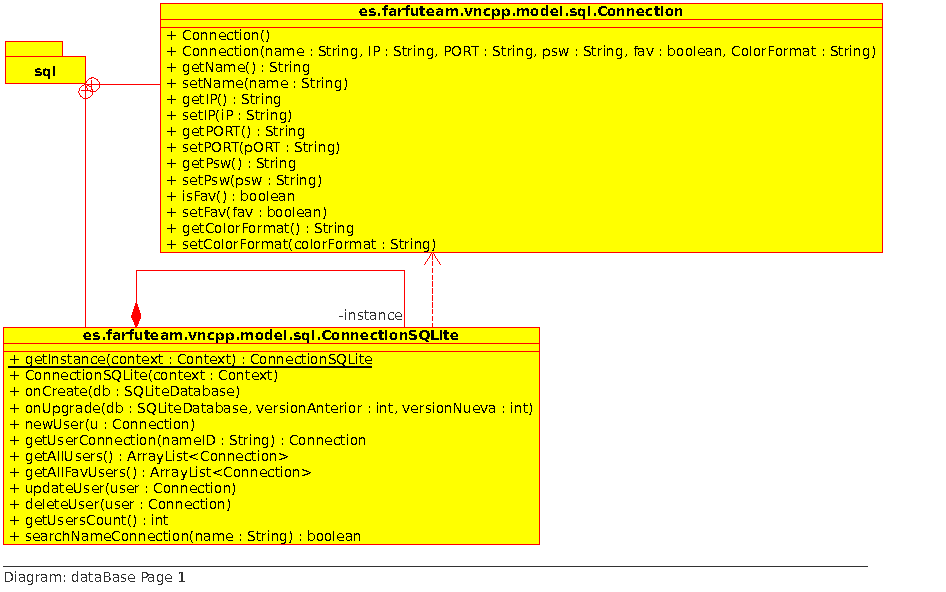
\includegraphics[scale=1]{BBDD.pdf}
\end{center}
\caption{Diagrama Base de Datos}
\end{figure}

La clase encargada de acceder a la base de datos (SQLite) es ConnectionSQLite (Ver Figura 6.1). Ésta es llamada desde diferentes Activities como NewConnectionActivity y EditionActivity. La clase Connection se utiliza como clase transfer con la información de una conexión.\\

ConfigurationMenu crea el menú de configuraciones. Como las clases anteriores es también llamada desde ActivityTabs. Si el usuario cambia alguna configuración, ConfigurationMenu llama al Singleton de Configuration y le pasa los valores que se hayan modificado.

\begin{figure}[h]
\begin{center}
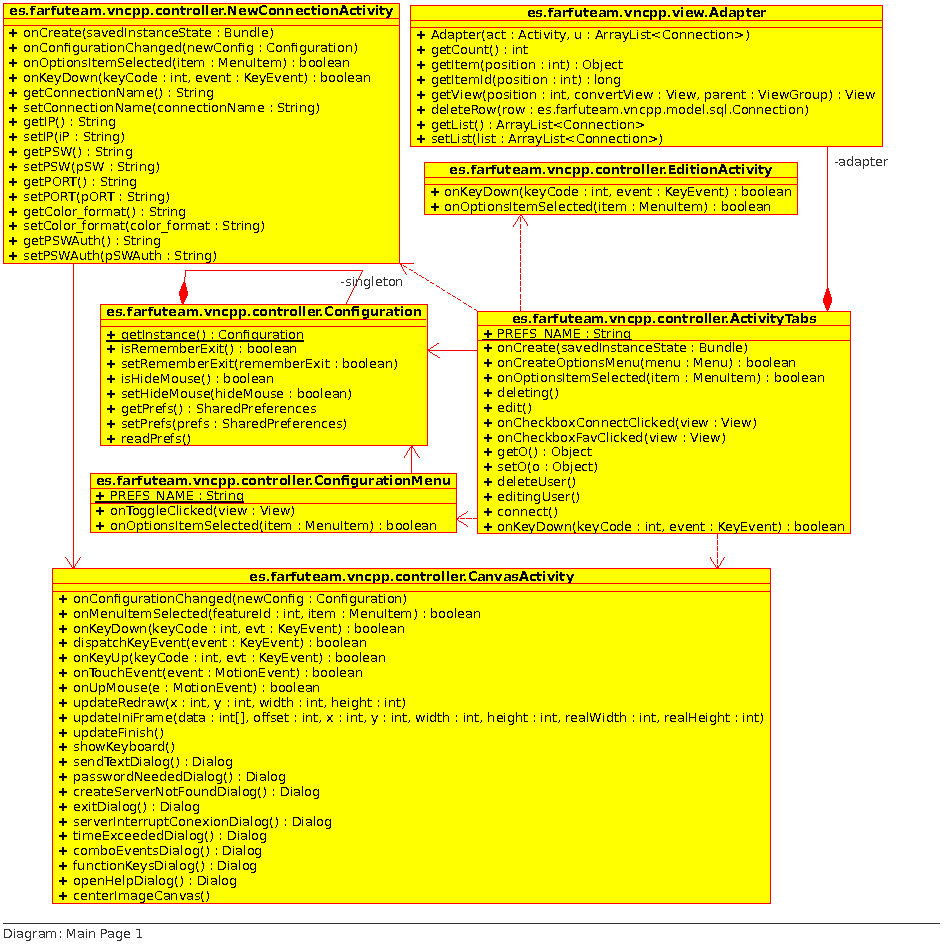
\includegraphics[scale=1]{Main.pdf}
\end{center}
\caption{Diagrama Activity Principal}
\end{figure}

Configuration es un singleton que se encarga de acceder al fichero de preferencias. ActivityTabs en el método onCreate llama a esta clase para que se instancie y cargue los datos de este fichero. Luego Configuration podrá ser llamado desde ConfigurationMenu si el usuario decide cambiar algo en la configuración de la aplicación.\\

Adapter es una clase que sirve para configurar cada elemento de la lista de conexiones y la lista de favoritos.\\

\begin{figure}[h]
\begin{center}
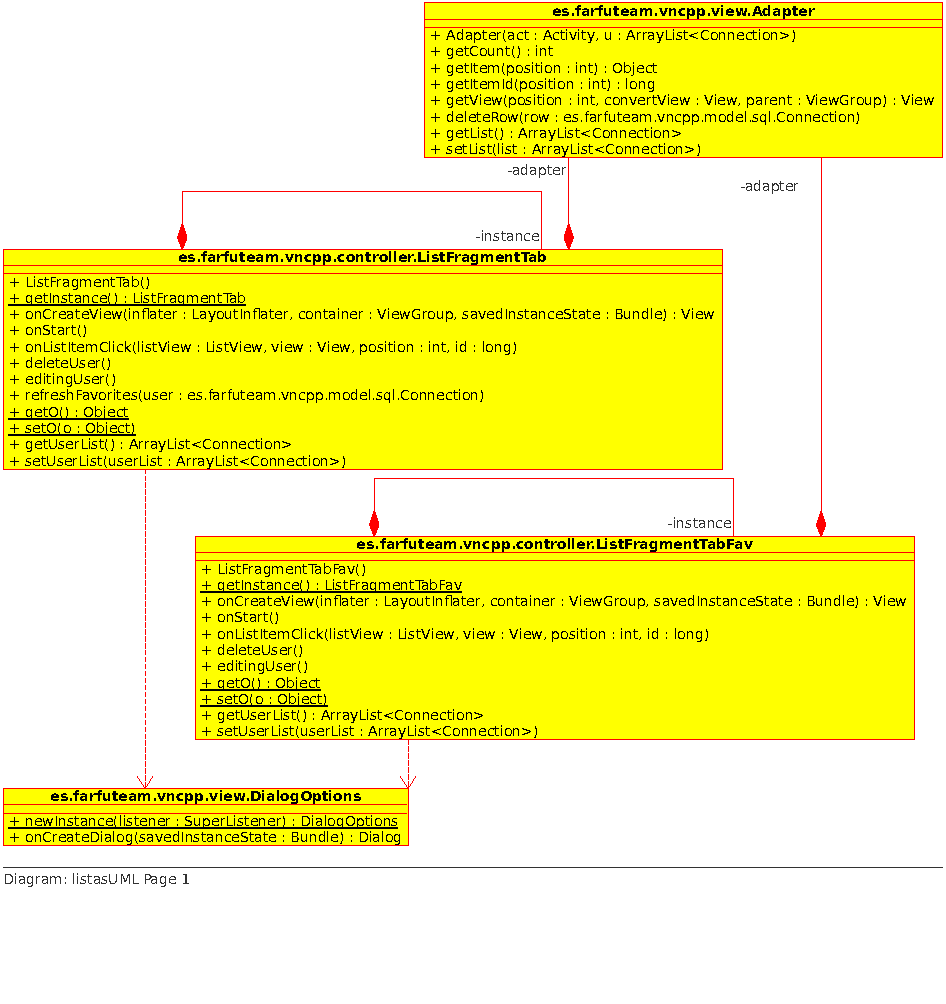
\includegraphics[scale=1]{Listas.pdf}
\end{center}
\caption{Diagrama Listas de Conexiones}
\end{figure}

Las clases ListFragmentTab y ListFragmentTabFav (Ver Figura 6.3) son las encargadas de mostrar las listas de conexiones y conexiones favoritas respectivamente.\\

La clase SlideListFragment (Ver Figura 6.4) se encarga de construir el menú lateral y es llamada desde CanvasActivity.\\

CanvasActivity (Ver Figura 6.4) es la encargada de capturar todos los eventos que se produzcan en el cliente, de mostrar la imagen del escritorio y de comunicarse con la parte nativa. Para dibujar la imagen se apoya en la clase CanvasView (Ver Figura 6.4). Para comunicarse con la parte nativa se apoya en VncBridgeJNI (Ver imagen 6.5). La comunicación entre el VncBridgeJNI y el CanvasActivity se realiza mediante el patrón observer (Ver figura 6.4 y 6.5).\\

\begin{figure}[h]
\begin{center}
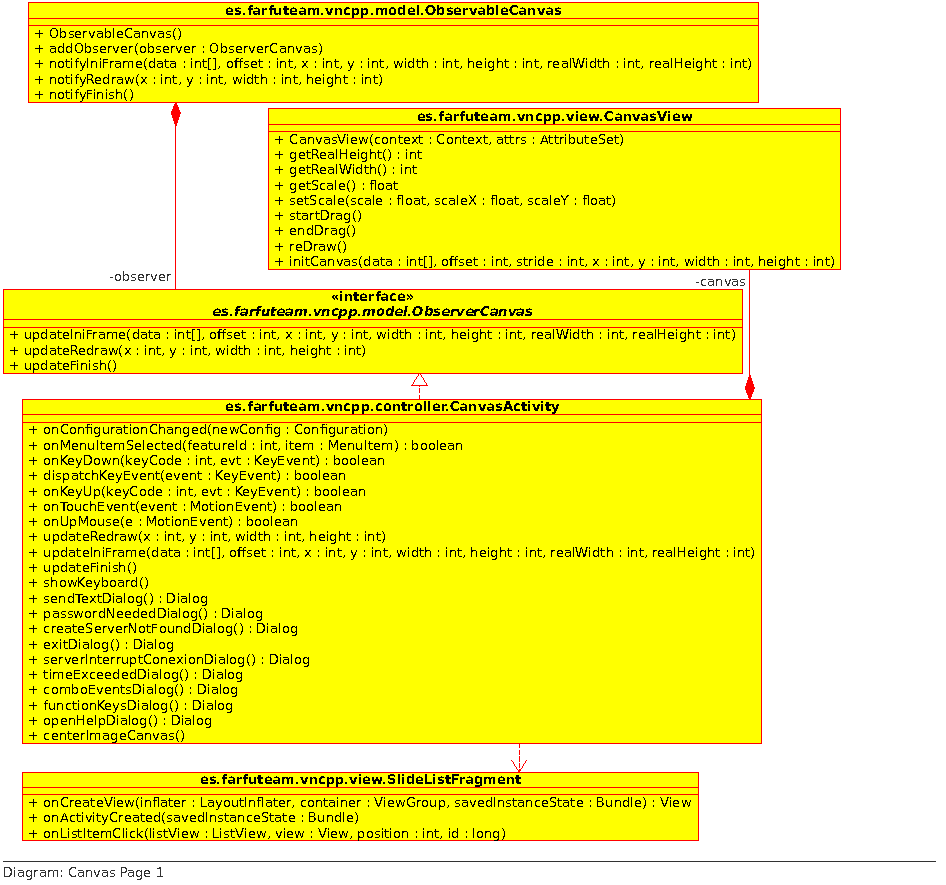
\includegraphics[scale=1]{Canvas.pdf}
\end{center}
\caption{Diagrama Canvas}
\end{figure}

La representación de la imagen se ha realizado con canvas, en la clase CanvasView (Ver Figura 6.4). Para dar mejor sensación de fluidez a la hora de moverse por la imagen se utiliza un Bitmap auxiliar en lugar de siempre el mismo. Cuando el programa entra en modo drag, se crea el Bitmap auxiliar y se inicializa con el valor actual de la imagen. Si el usuario está moviendose por la imagen (modo drag) el método \emph{onDraw} de canvas mostrará el Bitmap auxiliar.
\begin{lstlisting}
if(!drag){	
  canvas.drawBitmap(data,offset,stride,x,y,width,height,false,null);
}
else{
  canvas.drawBitmap(bitmap, bitmapRect, bitmapRect,null);
}
\end{lstlisting}
\newpage
En el momento que el usuario deja de moverse salta un timer creado en un hilo aparte, de tal manera que durante 0.5 segundos la imagen no se destruye (Ver sección 5.2.3).\\

La actualización de la imagen nos llega desde el código nativo (Ver sección 6.2.2). Cuando llega una notificación desde C++ de que la imagen ha sido modificada, el canvas se invalida y se redibuja.\\

Si CanvasActivity detecta un evento de Scroll (movimiento por la pantalla), se llama al método \emph{doScroll}. Este método calcula cuantos píxeles se ha movido el usuario en los ejes X e Y, comprobando que no se salga de la imagen. Una vez calculados se llama al método de canvas \emph{scrollTo} para que modifique la imagen.
\begin{lstlisting}
if(moveX != 0 || moveY != 0){
  realX = realX + (int)moveX;
  realY = realY + (int)moveY
  canvas.scrollTo((int)(realX*scaleFactor),
		          (int)(realY*scaleFactor));
}
\end{lstlisting}

Si CanvasActivity detecta un evento de Scale (zoom), se recalcula el factor de escala y dependiendo de si ha sido positivo o negativo, se llama al método \emph{scrollTo} de canvas directamente o al método \emph{doScroll}.
\begin{lstlisting}
if(isDo){
  if(factor > 1){		
    int moveX = (int)(x*scaleFactor);
    int moveY = (int)(y*scaleFactor);
    if(x < 0){
      moveX = 0;
      y = 0;
    }
    if(y < 0){
      moveY = 0;
      y = 0;
    }
    realX = (int)x;
    realY = (int)y;
    canvas.scrollTo(moveX,moveY);
  }else if(factor<1 ){
    int auxX = 0;
    int auxY = 0;
    if(x * scaleFactor > canvas.getRealWidth()){
      auxX = -100;
    }else{
      auxX = -10;
    }
    if(y * scaleFactor > canvas.getRealHeight()){
      auxY = -100;
    }else{
      auxY = -10;
    }
    doScroll(auxX, auxY);
  }
}
\end{lstlisting}

VncBridgeJNI es la clase que proporciona los métodos para comunicarse con la parte nativa. Es capaz de llamar a funciones nativas tales como iniConnect, mouseEvent, keyEvent, etc., de esta manera se establece la comunicación de Java a C/C++ (Ver sección 5.2.2). Las notificaciones llegan desde el código nativo a través de la interfaz ObserverJNI.

\begin{figure}[h]
\begin{center}
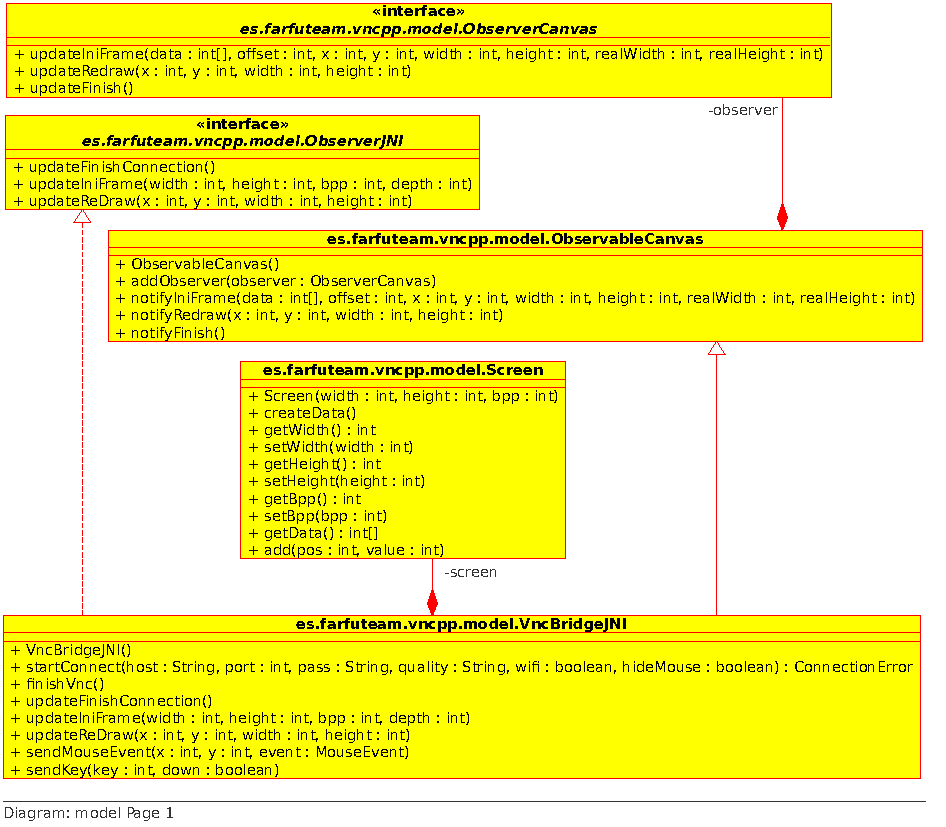
\includegraphics[scale=1]{Model.pdf}
\end{center}
\caption{Diagrama Modelo}
\end{figure}

\subsection{Parte escrita en C/C++}

Ahora vamos a describir el código escrito en C/C++. La clase Java VncBridgeJNI realiza las llamadas a la parte nativa a través de las funciones implementadas en el fichero JavaBridge.cpp. Este fichero no se muestra en el diagrama de clases puesto que no es una clase, aún así, su única función es hacer las llamadas propias a la clase Vnc, en otras palabras actúa como puente de Java a C++.

\begin{figure}[h]
\begin{center}
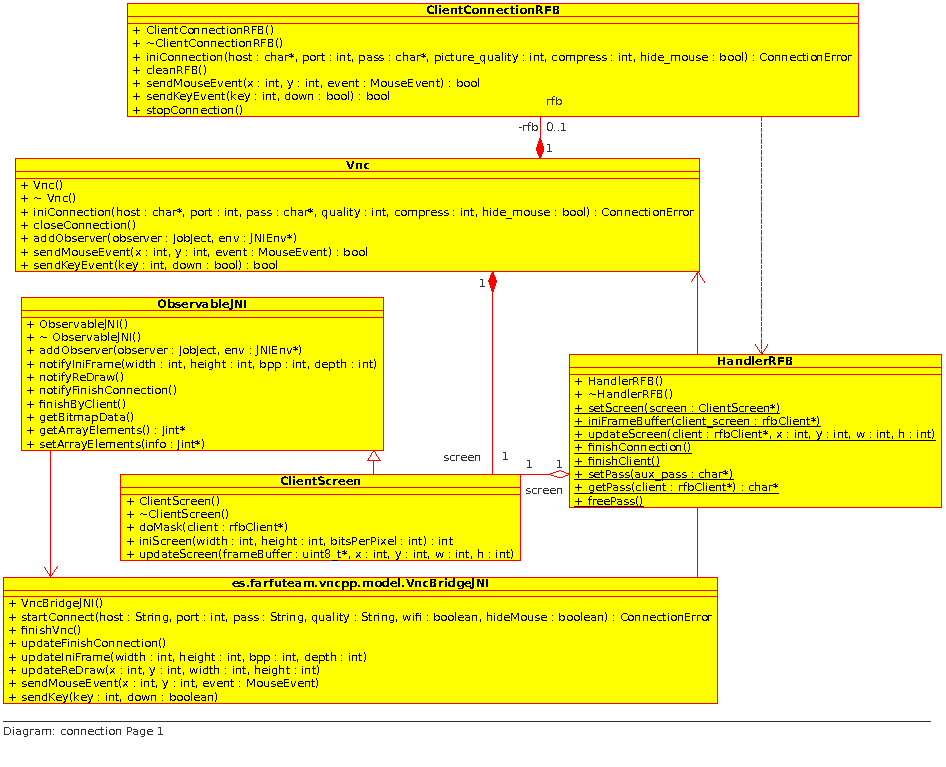
\includegraphics[scale=1]{Connection.pdf}
\end{center}
\caption{Diagrama Conexión}
\end{figure}

Al inicializar el código nativo se crea la clase Vnc (Ver Figura 6.6) y se añade el observer a la clase ClientScreen para que éste pueda realizar las notificaciones a Java. En la constructora de Vnc se crean las clases ClientScreen, ClientConnectionRFB y se le pasa a la clase HandlerRFB la referencia a ClientScreen para que ésta pueda comunicarse con ella. Vnc retrasmitirá todas las órdenes que le lleguen de JavaBridge a ClientConnectionRFB.\\

La clase ClientConnectionRFB (Ver Figura 6.6) es la encargada de gestionar la conexión entre el cliente y el servidor utilizando el protocolo RFB. Para establecer una conexión lo primero que se hace es inicializar la estructura rfbClient, en este punto se indica cual es el host, el puerto, la calidad de imagen, etc. Un punto muy importante de la inicialización es indicar cuales son las funciones que se han de llamar cuando el server mande notificaciones. Para ello nos apoyamos en la clase HandlerRFB, de tal manera que, por ejemplo, cuando llega un update de la imagen indicamos que tiene que llamar al método \emph{updateScreen} del handler.
\begin{lstlisting}
clientRFB=rfbGetClient(bitsPerSample,samplesPerPixel,bytesPerPixel);
clientRFB->serverPort = port;
clientRFB->serverHost = host;
clientRFB->programName = "VNC++";
HandlerRFB::setPass(pass);
clientRFB->GetPassword = HandlerRFB::getPass;
clientRFB->appData.qualityLevel = picture_quality;
clientRFB->appData.compressLevel = compress;
clientRFB->appData.useRemoteCursor = hide_mouse;
clientRFB->MallocFrameBuffer=HandlerRFB::iniFrameBuffer;
clientRFB->canHandleNewFBSize = TRUE;
clientRFB->GotFrameBufferUpdate=HandlerRFB::updateScreen;
clientRFB->FinishedFrameBufferUpdate= HandlerRFB::finishUpdate;
clientRFB->listenPort = LISTEN_PORT_OFFSET;
clientRFB->listen6Port = LISTEN_PORT_OFFSET;
\end{lstlisting}

Una vez terminada la inicialización de rfbClient se procede a la conexión con el servidor.
\begin{lstlisting}
if(!rfbInitClient(clientRFB,0,NULL)){
  error_connect = NoServerFound;
  if(DEBUG)
    LOGE("No server found");
  clientRFB = NULL;
}
else if( !clientRFB->frameBuffer){
  if(DEBUG)
    LOGE("No Frame Found");
  error_connect = NoFrameFound;
  cleanRfb();
}
\end{lstlisting}

Si todo va bien se crea un hilo para manejar los eventos del protocolo RFB. Dicho hilo es un bucle infinito a la espera de mensajes que provengan del servidor.
\begin{lstlisting}
while(!aux_this->stop_connection) {
  mes=WaitForMessage(aux_this->clientRFB,timeWait);
  if(mes<0){
    aux_this->stop_connection = true;
    serverOut = true;
  }
  if(mes){
    if(!HandleRFBServerMessage(aux_this->clientRFB)){
      aux_this->stop_connection = true;
      serverOut = true;
    }
  }
}
\end{lstlisting}

La variable aux\_this es un puntero a ClientConnectionRFB. Si no se ha parado la conexión se espera hasta que llega un mensaje del servidor, la función encargada de ello es \emph{WaitForMessage}. Después la función \emph{HandlerRFBServerMessage} es la encargada de comprobar cual es el mensaje que ha llegado y en función de ello, llamar a unas funciones u otras de HandlerRFB.\\

Para enviar los eventos del ratón o de pulsación de teclas se utilizan las funciones \emph{SendPointerEvent} y \emph{SendKeyEvent} respectivamente. Cabe destacar que para enviar el evento de pulsación de teclado hay que transformar el código de tecla que nos llega desde Java para que el server sea capaz de interpretarlo correctamente.
\begin{lstlisting}
bool ClientConnectionRFB::sendKeyEvent(int key,bool down){
  rfbKeySym rfbKey = transformToRfbKey(key);
  if(rfbKey != 0){
    SendKeyEvent(clientRFB,rfbKey,down);
  }
}
\end{lstlisting}

La clase HandlerRFB (Ver Figura 6.6) es una clase completamente estática. Esto se debe a que, dado que LibVNCServer se encuentra escrita en C y los eventos del mismo son punteros a funciones, si no fuesen estáticos los métodos en C++ tienen de forma implícita el parámetro this, que es una referencia a la propia clase. Por el contrario C no es un lenguaje orientado a objetos, por ello ese parámetro this no existe en las llamadas. Al declarar estáticos los métodos, el parámetro this desaparece. Sus métodos básicamente redirigen la llamada a las funciones de ClientScreen, por eso era necesario pasar la referencia al inicio.\\

ClientScreen (Ver Figura 6.6) se encarga del manejo de las actualizaciones de la imagen, así como de comunicar todos los cambios a Java. Esta comunicación la hace a través de ObservableJNI mediante la herencia de sus métodos.\\

Cuando llega un evento de inicializar la imagen desde el handler, se llama al método \emph{iniScreen}. En este método se inicializan todos los valores de la imagen y se envía una notificación a Java.
\begin{lstlisting}
int ClientScreen::iniScreen(const int width,
			    const int height,
			    const int bitsPerPixel) {
  if(DEBUG)
    LOGE("JNI iniFrameBuffer");
  this->width=width;
  this->height=height;
  //se pasa de bits a byte
  this->bytesPerPixel=bitsPerPixel/8;
  this->depth = bitsPerPixel;
  //se calcula el espacio total del buffer
  this->size = this->height*this->width*this->bytesPerPixel;
  if(DEBUG)
    LOGE("FIN JNI iniFrameBuffer");
  notifyIniFrame(this->width,
		 this->height,
		 this->bytesPerPixel,
		 this->depth);
  return size;
}
\end{lstlisting}

Cuando se quiere invocar métodos de Java, para notificar cambios, es necesario colocarse en el entorno de ejecución actual, esto es, en el hilo. Para ello usamos la función \emph{getEnviroment}. Este método comprueba si la variable env, del tipo JNIEnv*, se encuentra apuntando al hilo actual, si no fuese el caso, se coloca en él.

\begin{lstlisting}
void ObservableJNI::getEnviroment(){
  int getEnv = vm- >GetEnv((void**)&env,JNI_VERSION_1_6);

  if(getEnv == JNI_EDETACHED){
    vm->AttachCurrentThread(&env,NULL);
  }
}
\end{lstlisting}

El método notifyIniFrame obtiene el método \emph{updateIniFrame} del entorno Java y lo llama pasándole la información nueva. Después se llama a \emph{GetObjectClass} para obtener la clase VncBridgeJNI y así, poder hacer llamadas a sus métodos. Para hacer una llamada a un método de Java, una vez tenemos la clase, hay que utilizar el método \emph{GetMethodID} para obtener el ID del método que deseamos invocar. Una vez que dispongamos de dicha ID podemos llamarlo usando \emph{CallVoidMethod}.
\begin{lstlisting}
void ObservableJNI::notifyIniFrame(int width,
				   int height,
				   int bpp,
				   int depth){
  getEnviroment();
  if(DEBUG)
    LOGE("Take method iniFrame");
  observer_class  = env->GetObjectClass(this->observer_object);
  //cogemos el ID
  jmethodID updateScreen = env->GetMethodID(observer_class,
					    "updateIniFrame",
					    "(IIII)V");
  if(DEBUG)
    LOGE("Launch method iniFrame");
  env->CallVoidMethod(observer_object,
		      updateScreen,
		      width,
		      height,
		      bpp,
		      depth);
  if(DEBUG)
    LOGE("Finish launch method iniFrame");
  env->DeleteLocalRef(observer_class);
}
\end{lstlisting}

Para finalizar, el método \emph{updateScreen} de ClientScreen es el encargado de actualizar una porción de la imagen. El inicio de la porción a actualizar viene indicado por los parámetros x e y, siendo w y h la anchura y la altura respectivamente de dicha porción.
\begin{lstlisting}
void  ClientScreen::updateScreen(uint8_t *frameBuffer,
				 const int x,
				 const int y,
				 const int w,
				 const int h){
  if(DEBUG)
    LOGE("JNI Update");
  int pixel;
  int pos;
  int pos_col;
  int pos_array;
  getBitmapData();
  jint *info = getArrayElements();
  int real_i,real_j;
  for(int i=0;i < w;i++ ){
    real_i = i + x;
    pos_col = (real_i*bytesPerPixel);
    for(int j=0;j<h;j++){
      real_j = j + y;
      pos = ((bytesPerPixel*width) * real_j) + pos_col;
      memcpy(&pixel,&frameBuffer[pos],bytesPerPixel);
      pos_array = (width *real_j) + real_i;
      info[pos_array] = pixel;
    }
  }
  if(DEBUG)
    LOGE("JNI notify reDraw");
  setArrayElements(info);
}
\end{lstlisting}

Lo que hace este método es recorrer la porción que ha cambiado con los dos bucles for. Las variables real\_i y real\_j son las posiciones reales de la porción dentro de la imagen. Como la imagen se representa en un buffer unidimensional es necesario calcular el desplazamiento que se obtiene:

\begin{equation*}
pos = ((bytesPerPixel)(width))(real\_j)+((real\_i)(bytesPerPixel))
\end{equation*}

Una vez tenemos la posición copiamos el píxel con memcpy y lo guardamos en info. El bitmap info es una referencia al bitmap de Java, lo obtenemos a través de los métodos \emph{getBitmapData} y \emph{getArrayElements}, de tal manera que cuando se modifican elementos de dicho bitmap en C se están modificando en Java. Lo único que falta por hacer es actualizar la información a través del método \emph{setArrayElements}. Mediante el que JNIEnv libera el vector del entorno de C/C++ con la función  \emph{ReleaseIntArrayElements} y se actualiza el vector de Java. 
